\documentclass[12pt]{article}
\usepackage[margin=2cm]{geometry} 
\usepackage{titling}
\usepackage{graphicx}
\usepackage{float}
\usepackage[hidelinks]{hyperref}
\usepackage{subcaption}

\setlength\parindent{0pt}
\setlength{\droptitle}{-2.8cm}

\title{Project report - Movie search}

\author{Stefano Taillefert\\
Information Retrieval}

\date{\today}


\begin{document}
\maketitle

\tableofcontents

\newpage

\section{Introduction}

	\subsection{Requirements}
	
	Movie search: you have to build a system that crawls movie websites like IMDb, RottenTomatoes, allmovie.com etc. for movies produced in the last ten years. The system has to
provide an interface for searching movies by title, browsing, and presenting the results. Besides that, the system should have results clustering: the system should group movies into genres (if a movie is labelled with multiple genres assign it the first one mentioned on the websites). There should be a possibility for expanding/shrinking a genre to show all the movies related to the genre. In addition, genres should be sorted in a descending order by the number of relevant movies under them.
	
	\subsection{Development}
	
		I started concretely working on this project on the 17th of October with the first commit, the boilerplate for the UI web app. Then, by the half of November I had added the crawlers and Solr's binaries to start working on the data as well. From there, it has been a cycle of continuously fixing existing bugs and progressively integrating new features.\\
		
		Overall, it has been a very nice experience and I learned to use a wide range of new tools and to integrate existing ones with new technologies to develop new functionalities.
	
	\subsection{Problems and known limitations}
	
		I had originally left the crawlers to work until they terminate, and the IMDb one ran for three days collecting around 3.5 million results. The generated JSON file was around 1 GB in size, making it too big to push it to GitHub; therefore, I had to integrate Git-LFS to support bigger files. Unfortunately this complicated the repo cloning for the end users and Solr was taking way too much to index the data, so in the end I decided to shrink my dataset to ca. 50'000 entries, which is still a robust amount but in the reasonable limits.\\
		
		There is a weird bug that prevents me from firing the search event when the user presses enter on the keyboard. It started happening after adding the genre selection menu to the main page but I'm not sure why. Since it came up quite at the end, I deemed it acceptable and didn't allocate too much time to look into it, having other more important features to polish.\\
	
		Last and definitively least, the website is clearly not responsive. I didn't pay attention to that part since it wasn't explicitly required, but a complete redesign would be required to make it usable on mobile (tables are generally a pain to work with on small screens).
	
	\newpage
	
	
\section{Tech stack and configuration}

	As many modern applications, this project has been separated in two components: frontend, which is the user-facing end offering the input fields and the result list, and backend, which is the ``brain" doing all the indexing and lookup. Another important part, but separated from the rest, are the crawlers, used to fetch the data from the web. Each component is detailed in the next subsections.
	
	\subsection{Crawlers}
	
		While this is not really a part of the final application, they are essential to gather the data. Built with Scrapy, there is a spider for each major movies website: IMDb, allmovie.com and RottenTomatoes. They are all configured to gather the same data: movie title, description (except for allmovie), genre, year, image, rating and link. They have some limitations, though: the image fetching doesn't work since all the websites use JavaScript to load them and Scrapy doesn't natively execute JS code. The only solution would be to set up a headless browser and have that one navigate the page, then grab the images from there. While it would be a nice feature to have, it seemed quite complicated and I preferred to focus on more essential parts of the project. The same problem goes for the whole RottenTomatoes website, which is basically completely dynamically loaded. As that was the third site in my list, I thought that two sources might be enough for my dataset: in the end, to crawl another website you just need to put the right URL and CSS elements to extract the information you need.\\
		Another known limitation is that the entries from allmovie don't have a description, since it's not on the main page with the rest of the data; to fetch that value as well, I would need to open each and every movie page, which would add a significant overhead to the crawling operation.		
	
	\subsection{Frontend}
	
		The part responsible of displaying the user interface has been created with React. I went for the simplest approach, cramming everything in one single file and choosing a single-page design. The structure is based on Material-UI and has been kept as minimal and compact as possible. The query operations (performed either through the genre selector or the search bar) trigger a GET request to the backend's endpoints, which are detailed in the next section.	
	
	\subsection{Backend}
	
		This is the backend of our application, running on Solr 8.7.0. It has to index and store all data that the user has previously crawled, while offering some endpoints to retrieve the collection (or optionally update it). The queries are mainly made on the \texttt{/select} route, passing along the various parameters like genre, sorting and index of the results page. The schema has been manually crafted to ensure a good representation of our data at all times, while the indexing and model settings have been left to default since they seem to work pretty well in my case.
		
	\newpage
	
	\subsection{Docker}
	
		Probably too much time has been put into this completely not required part, but I really like dockerizing applications. For this project, two containers were necessary, one for each of the components mentioned earlier. The configuration for the frontend was quite straightforward, since containerizing frontends is a quite common practice, especially for React apps. Luckily I found out that Solr already has an official image, but the setup was quite the journey. I had to copy the configset to the container through Docker volumes and have it run some script on startup to correctly create the node. Then, as instructed in the \texttt{README}, the user must execute a command to index their data. Not the prettiest solution, but I think it's a good compromise between a premade solution and user input. Of course, running the project in a Docker environment added the challenge of networking due to different hostnames, requiring an additional proxy on the client side to detect if the UI is running on bare metal or in a container, thus proxying the requests respectively to \texttt{localhost} or \texttt{ir-project\_solr} (aka the Solr container).
		
		\begin{figure}[H]
			\centering
			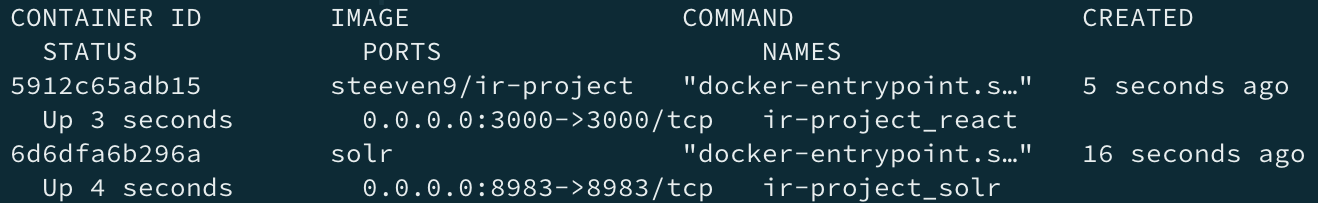
\includegraphics[width=\textwidth]{img/docker.png}
			\caption{The docker containers running}
			\label{img:docker}
		\end{figure}
	
	\newpage
	
	
\section{User interface}\label{sec:UI}

	The very first version had only a search bar and the table to display the result, basically like in figure \ref{fig:interfaceOld1} but without the tabs, since I started working on a small subset of features first to start experimenting with all the technologies involved. Once that was working - and it took quite a while to figure out how to retrieve and parse the results correctly - I started adding features. For example, I completely customized the pagination system: since Solr by default sends only the first ten results and sending the whole results array was too expensive, I added two buttons and a local index variable to keep track of the current page the user is viewing. On each page load, the frontend asks Solr to send along the next (or previous) ten results, allowing for a fast initial loading and optimizing the network and memory usage.\\
	
	Once the searching part was done, I started working on the clustering part. Now, you should know that Solr has an embedded clustering feature that uses some pre-made algorithms (like Lingo) to cluster the results automatically. The official documentation provides some examples on how to use it and it seems quite straightforward; add some lines to the configuration file, specify the fields you want to cluster and you're done.\\
	
	Oh, if only it was that easy.\\
	
	With the clustering component enabled, Solr throws a \texttt{NullPointerException} (yes, it's built with Java) when creating the core. I lost literal \textit{weeks} trying to figure out why and I am ashamed to admit that to this day, I still have no idea. Some classmates and Ivan, our teaching assistant (blessed his soul!), have also looked into it, allowing me to test my config on their setup which promptly exploded just as mine.\\
	
	In the end, instead of bashing my head to make this feature work, I took a different approach: to allow the user to navigate through the genres as required, I added a section of the website (under the \texttt{Browse} tab, see figure \ref{fig:interfaceOld2}) with a list of genres to pick from.\\
	
	Following feedback from one of the evaluators, I later changed the design and merged the two tabs in one single interface to allow both searching for a specific term or browsing the catalog by genre. The selector on the left works in combination with the search bar if a query is inserted, allowing the user to refine their query as well.\\
	
	A note on the genre selector: while the specifics required the genres to be sorted by number of movies under them (in decreasing order), I personally found it to be really unpractical to select a genre.
	Therefore, I opted for a normal alphabetical order, leaving the amount of movies per genre next to it; this way, the user can look up the genres normally while still seeing which ones are more popular.
	
	\newpage
		
	\begin{figure}[H]
		\centering
		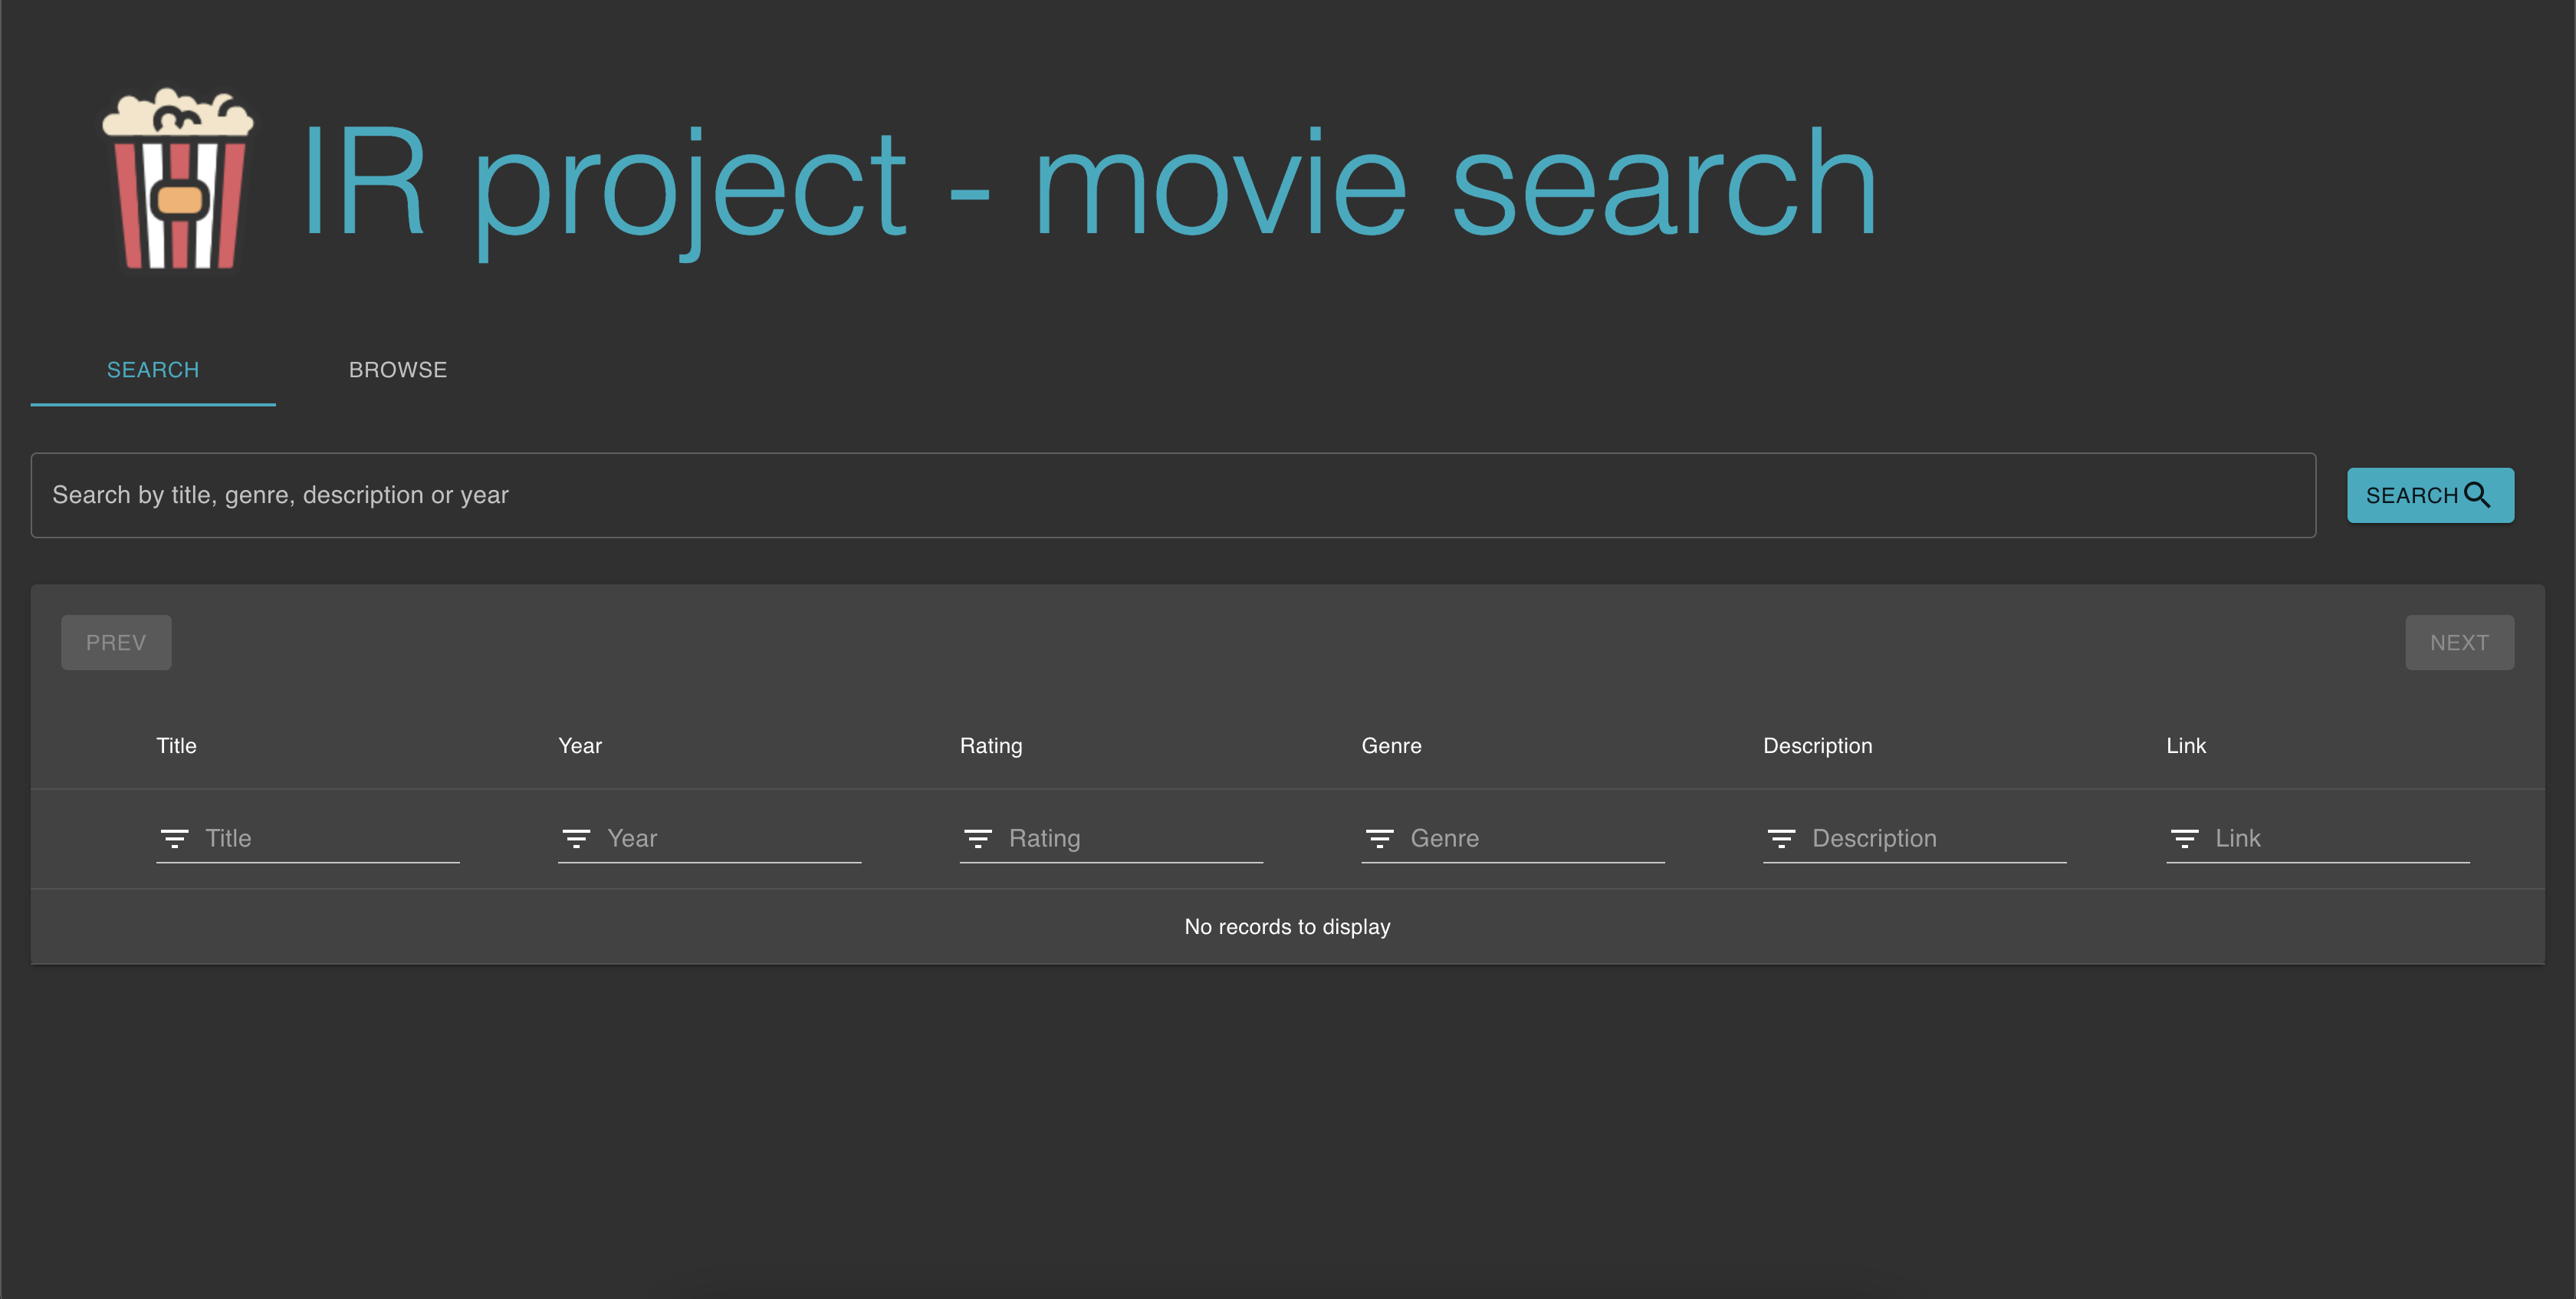
\includegraphics[width=\textwidth]{img/interfaceOld1.png}		
		\caption{The old user interface (v1.0.0) - search mode}
		\label{fig:interfaceOld1}
	\end{figure}
	
	\begin{figure}[H]
		\centering
		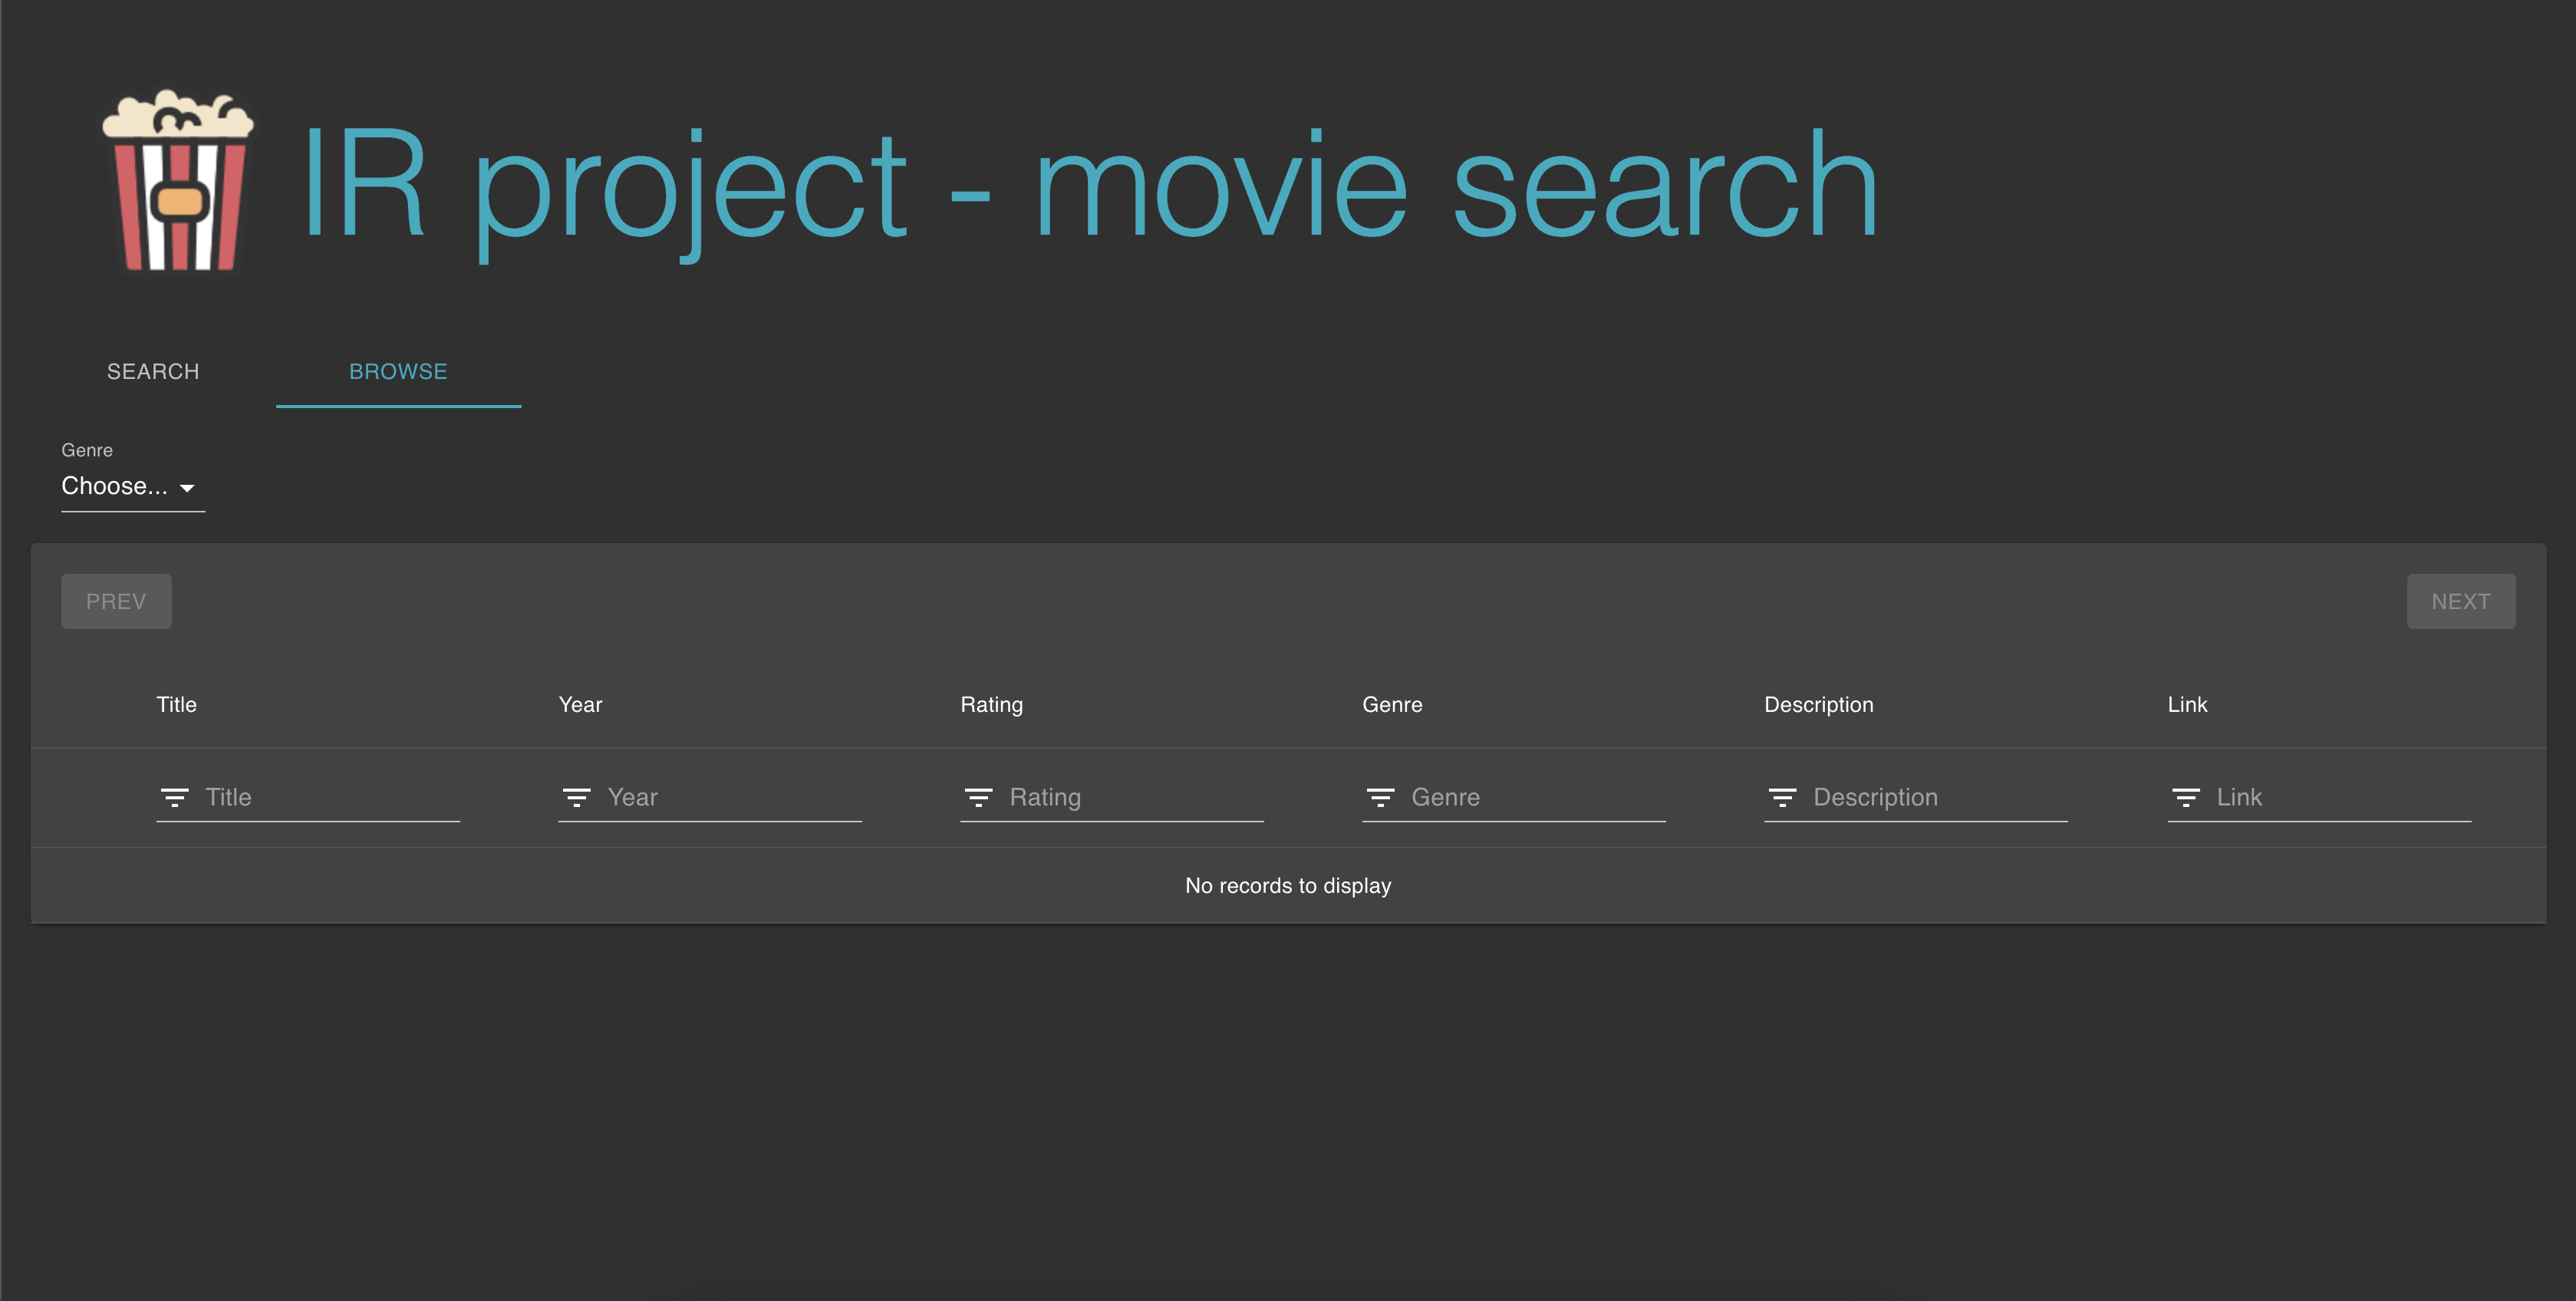
\includegraphics[width=\textwidth]{img/interfaceOld2.png}
		\caption{The old user interface (v1.0.0) - browse mode}
		\label{fig:interfaceOld2}
	\end{figure}
	
	\begin{figure}[H]
		\centering
		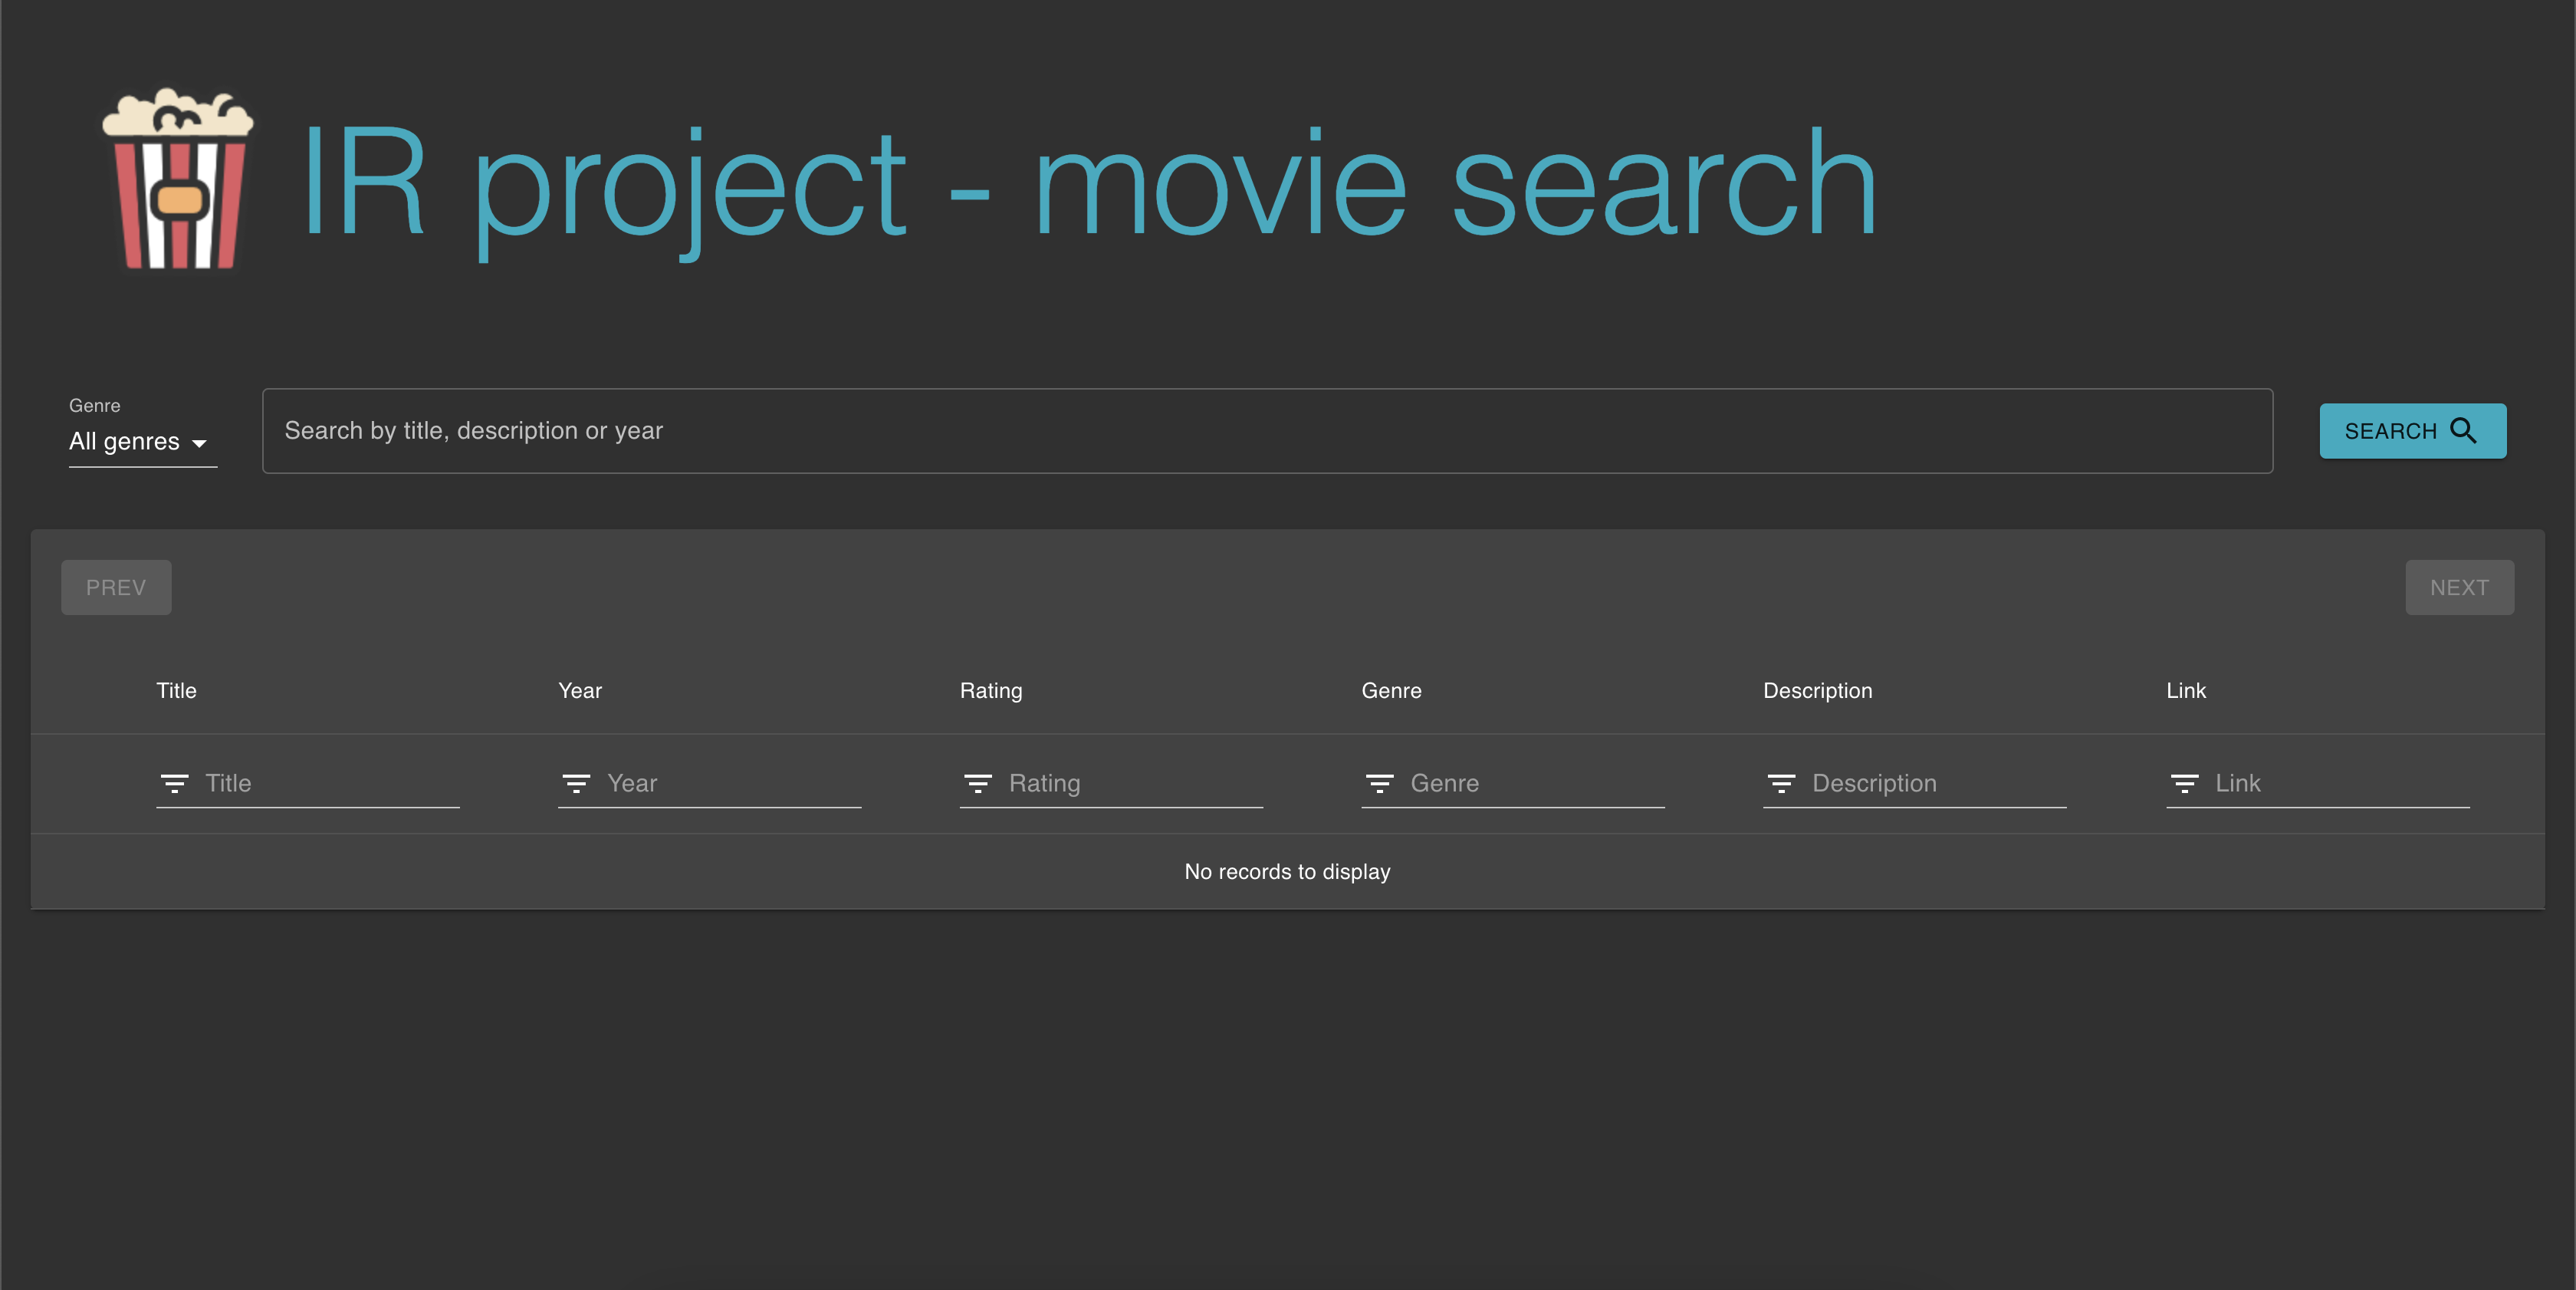
\includegraphics[width=\textwidth]{img/interface.png}
		\caption{The unified user interface (v1.1.0)}
		\label{fig:interface}
	\end{figure}
	
	\begin{figure}[H]
		\centering
		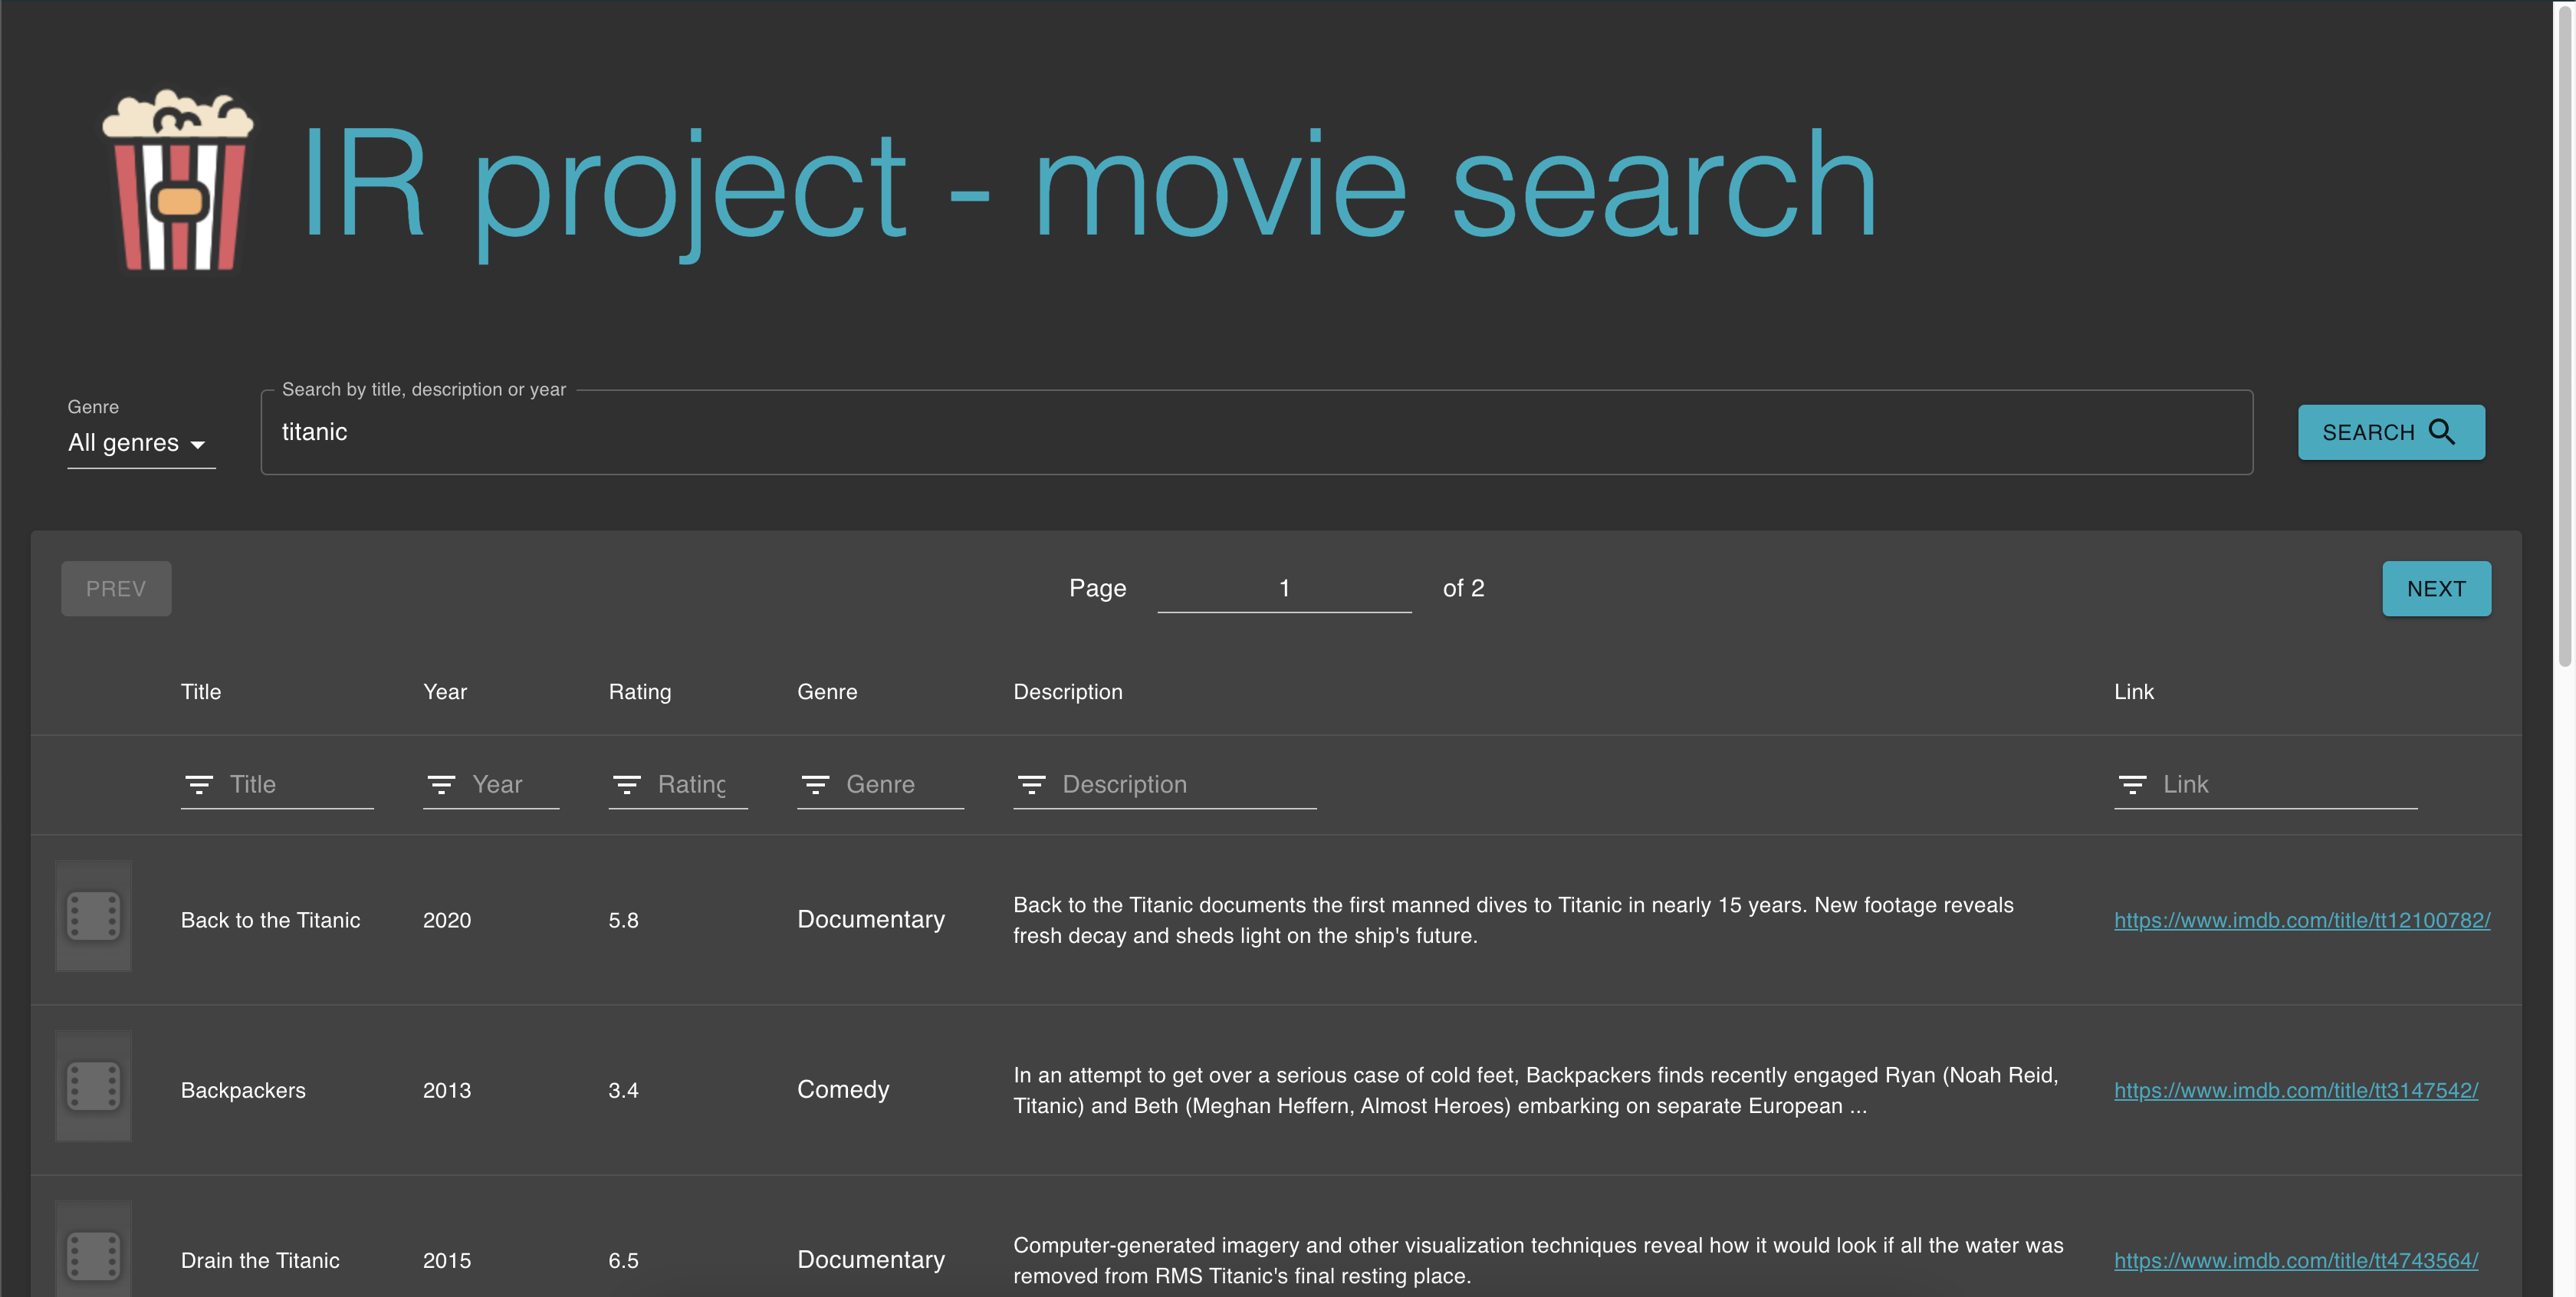
\includegraphics[width=\textwidth]{img/results.png}
		\caption{The search results (v1.1.0)}
		\label{fig:results}
	\end{figure}
	
	\newpage
	

\section{User evaluation}

	As required, I ran a user evaluation with three people, all fellow informatics students. All evaluators were provided with version 1.0.0 and were tasked with the following queries:
	
	\begin{itemize}
		\item find the movie ``Titanic"
	
		\item find all documentaries about the Titanic
	
		\item find all movies made in 2003
	
		\item get the list of all drama movies	
	\end{itemize}
	
	The first two evaluations were pretty much in line with each other: both users found the website really easy to use, ``intuitive and with many useful features". 
	Both suggested some minors tweaks, for example adding a link to the original movie page, and pointed out some bugs, for example with the page counting index. During the second evaluation, we also realized that the text search was providing some incorrect results (e.g. movies made in 2020 when looking for ``2003") and after some digging, I found a mistake in the Solr configuration (the copyField was including the document ID, which is an alphanumerical string). So the evaluations have been extremely useful also for debugging purposes! All the problems have been fixed right before the next evaluation to prevent redundant feedback.\\
	
	The third evaluator, on the other hand, suggested a UI overhaul since the two tabs were, in their opinion, redundant. The main idea was that the search box could be combined with the genre selection, removing the need for tabs and thus streamlining the UI. I agreed with their suggestion and this resulted in version 1.1.0, which is the latest one (see section \ref{sec:UI} for screen captures).\\
	
	
\section{Additional resources}

	GitHub repository: \url{https://github.com/Steeven9/IR-project}\\
	
	Docker repository: \url{https://hub.docker.com/repository/docker/steeven9/ir-project}\\
	
	Official Solr image: \url{https://hub.docker.com/_/solr}\\
	
	Scrapy documentation: \url{https://docs.scrapy.org/en/latest}\\
	
	React documentation: \url{https://reactjs.org/docs/getting-started.html}\\
	
	Material-UI documentation: \url{https://material-ui.com/getting-started/installation}\\
	
	Docker documentation: \url{https://docs.docker.com}\\
	
	Solr documentation: \url{https://lucene.apache.org/solr/guide/8_7}
	

\end{document}
